\subsection{Iconix}

\par O Iconix foi escolhido como a metodologia de desenvolvimento de \textit{software}, desempenhando um papel fundamental na organização. Sua abordagem proveu uma sequência de procedimentos, levando à construção de uma aplicação estável. Como relatado no quadro teórico, foram seguidas as quatro fases definidas pelo Iconix,

\par Na primeira fase, definida como análise de requisitos, foi realizado o levantamento das informações pertinentes ao desenvolvimento. Este levantamento foi realizado por meio da observação do comportamento das pessoas ao buscar por mão de obra temporária. A partir daí, foram levantadas as principais características, indispensáveis para a construção do \textit{software} e desenvolvido o modelo de domínio inicial, como demonstra a Figura~\ref{fig:modelo_dominio_inicial}.

\newpage
\begin{figure}[h!]
	\centerline{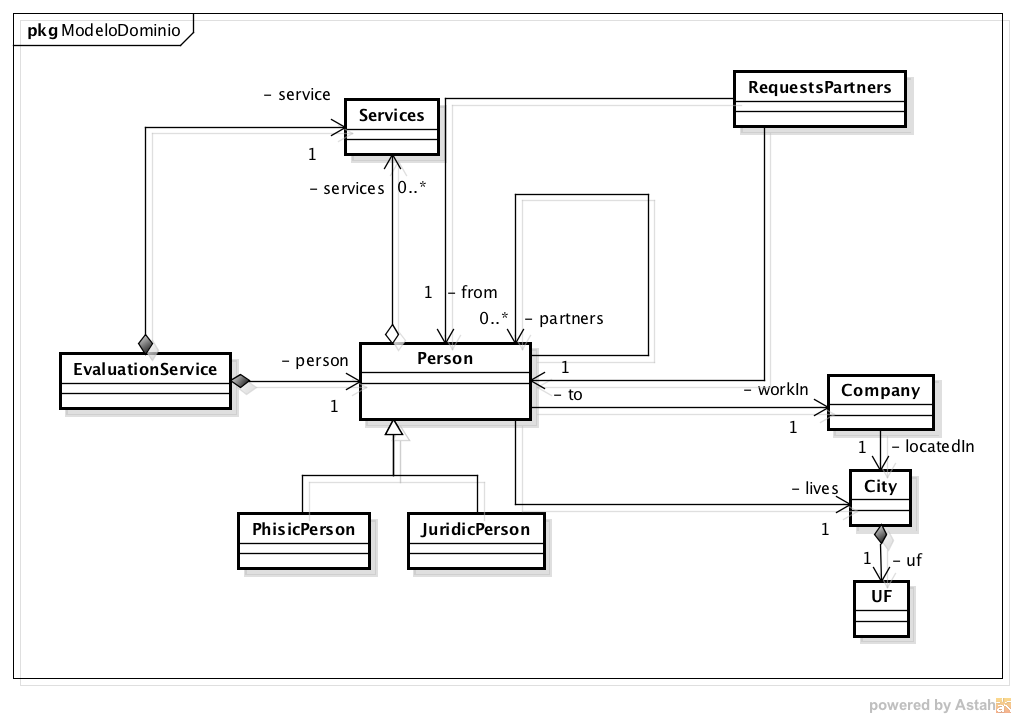
\includegraphics[scale=0.45]{./imagens/modelo-dominio-inicial.png}}
	\caption[Modelo de domínio inicial]
	{Modelo de domínio inicial. \textbf{Fonte:} Elaborado pelos autores.}
	\label{fig:modelo_dominio_inicial}
\end{figure}

\par Nesta fase, também foram definidas todas as ações cujo usuário poderia realizar no sistema, por meio dos casos de uso, conforme a Figura~\ref{fig:caso_uso_unificado}.

\newpage
\begin{figure}[h!]
	\centerline{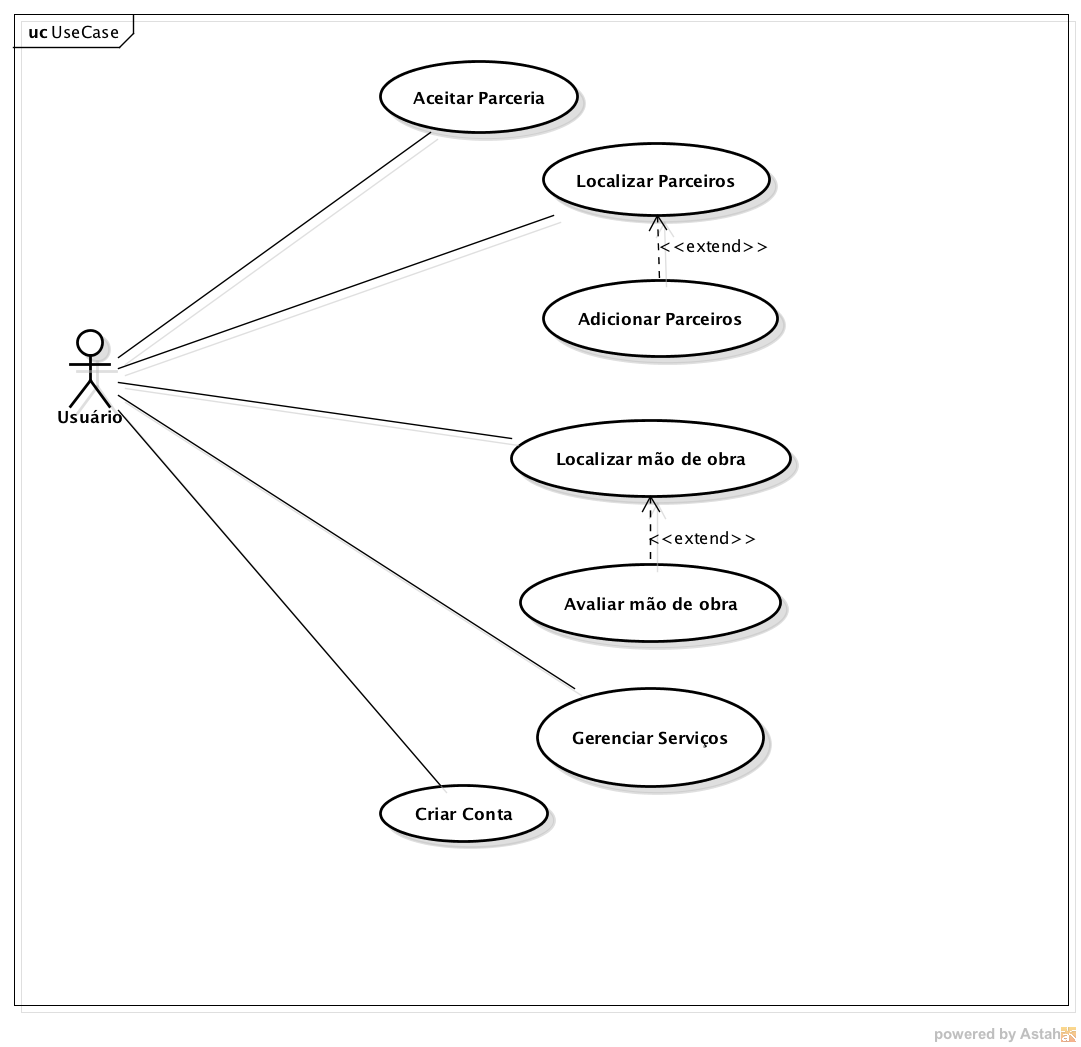
\includegraphics[scale=0.5]{./imagens/caso-de-uso-unificado.png}}
	\caption[Diagrama de caso de uso]
	{Diagrama de caso de uso. \textbf{Fonte:} Elaborado pelos autores.}
	\label{fig:caso_uso_unificado}
\end{figure}

% Removido após a pré-banca, pois, agora só haverá apenas um tipo de usuário (Ambos) e não mais provedor de serviço e contratante
%\newpage
%\begin{figure}[h!]
%	\centerline{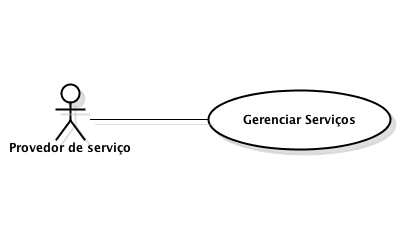
\includegraphics[scale=0.6]{./imagens/caso-de-uso-provedores-servico.png}}
%	\caption[Diagrama de caso de uso para provedores de serviços]
%	{Diagrama de caso de uso para provedores de serviços. \textbf{Fonte:} Elaborado pelos autores.}
%	\label{fig:caso_uso_provedor_servico_inicial}
%\end{figure}

%\begin{figure}[h!]
%	\centerline{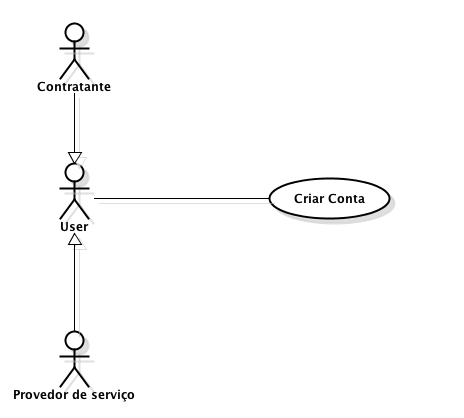
\includegraphics[scale=0.6]{./imagens/caso-de-uso-usuario.png}}
%	\caption[Diagrama de caso de uso para contratantes e provedores de serviços]
%	{Diagrama de caso de uso para contratantes e provedores de serviços. \textbf{Fonte:} Elaborado pelos autores.}
%	\label{fig:caso_uso_usuario_inicial}
%\end{figure}

\par Após definir os casos de uso, foram escritos os fluxos de eventos, para cada caso de uso. A seguir será apresentado o fluxo de eventos relacionado ao caso de uso ''Localizar parceiros'' por meio do Quadro~\ref{quad:fluxo_evento_localizar_parceiro}. Os demais fluxos de eventos são apresentados no Apêndice I em conjunto com os outros digramas gerados por este trabalho.

% Conferir com o Márcio se os quadros serão removidos daqui e colocados nos apêndices depois só colar esta parte onde for inserida
%\newpage
%\begin{quadro}[h!]
%	\begin{fluxoDeEventos}
  \addTitle{Localizar Mão de obra}
  \addrow{Ator principal}{Contratante ou Ambos}
  \addrow{Ator secundário}{-}
  \addrow{Pré-condições}{O ator estar autenticado no sistema}
  \addrow{Pós-condições}{Provedores de serviço e suas respectivas mão de obras apresentadas ao ator.}
  
  \startBasicFlow{Ator} {Sistema}
  \addItemByColumnOne{O ator acessa a página para buscar o serviço por meio do menu “Busca” localizado no menu principal do sistema.}
  \addItemByColumnTwo{O sistema apresenta a página de busca de serviço e mão de obra.}
  
  \addItemByColumnOne{O ator informa qual a mão de obra que ele deseja pesquisar, por meio do campo “Buscar serviço”.}
  \addItemByColumnTwo{O sistema realiza uma busca pelo serviços que possuem o nome parecido com o nome do serviço informado pelo ator.ceiros que possuem maior probabilidade de se juntar a sua rede de parceiros.}
  
  \addItemByColumnOne{O ator seleciona o serviço a qual ele deseja que sejam pesquisados os provedores de serviço.}
  \addItemByColumnTwo{O sistema irá realizar a busca pela mão de obra solicitada pelo ator em sua base de dados, levando em consideração a rede de parceiros do ator, a empresa onde ele trabalha e a cidade onde o ator vive. Além é claro, da qualificação dos provedores de serviço. Após esta busca, o sistema apresentará uma página com a lista de prestadores de serviço que prestam tal mão de obra, ordenada pela credibilidade em sua rede de parceiros.}
  
  \addItemByColumnOne{O ator analisa a lista e seleciona a melhor opção a ele, clicando em sua imagem de perfil.}
  \addItemByColumnTwo{O sistema pesquisa todas as informações restantes do provedor de serviço, selecionado, pelo ator e apresenta uma página contendo todas as informações do provedor selecionado.}
   
  \startAlternativeFlow{Fluxo alternativo 1}
  \noAlternativeFlow{Não há fluxos alternativos}
\end{fluxoDeEventos}

%	\caption[Fluxo de eventos para o caso de uso ''localizar mão de obra'']
%	{Fluxo de eventos para o caso de uso ''localizar mão de obr''. \textbf{Fonte:} Elaborado pelos autores}
%	\label{quad:fluxo_evento_localizar_mao_de_obra}
%\end{quadro}

%\begin{quadro}[h!]
%	\begin{fluxoDeEventos}
  \addTitle{Avaliar Mão de obra}
  \addrow{Ator principal}{Contratante ou Ambos}
  \addrow{Ator secundário}{-}
  \addrow{Pré-condições}{O ator estar autenticado no sistema}
  \addrow{Pós-condições}{Mão de obra avaliada pelo ator}
  
  \startBasicFlow{Ator} {Sistema}
  \addItemByColumnOne{Após o item 6 do fluxo principal do fluxo de eventos “Localizar Mão de obra”. O ator clica no botão “Avaliar Serviço”.}
  \addItemByColumnTwo{O sistema apresenta o formulário de avaliação na mesma página para o ator.}
  
  \addItemByColumnOne{O ator preenche o formulário de avaliação da mão de obra e clica no botão “Salvar”.}
  \addItemByColumnTwo{O sistema registra a avaliação do cliente e apresenta uma mensagem de sucesso a ele.}
   
  \startAlternativeFlow{Fluxo alternativo 1}
  \noAlternativeFlow{Não há fluxos alternativos}
\end{fluxoDeEventos}

%	\caption[Fluxo de eventos para o caso de uso localizar mão de obra]
%	{Fluxo de eventos para o caso de uso localizar mão de obra. \textbf{Fonte:} Elaborado pelos autores}
%	\label{quad:fluxo_evento_avaliar_mao_de_obra}
%\end{quadro}

\newpage
\begin{quadro}[h!]
	\begin{fluxoDeEventos}
  \addTitle{Localizar Parceiros}
  \addrow{Ator principal}{Contratante ou Ambos}
  \addrow{Ator secundário}{-}
  \addrow{Pré-condições}{O ator estar autenticado no sistema}
  \addrow{Pós-condições}{Possíveis parceiro(s) apresentado(s) ao ator}
  
  

  \startBasicFlow{Ator} {Sistema}
  \addItemByColumnOne{O ator clica no menu “Rede de Parceiros” no menu principal localizado no menu principal do sistema.}
  \addItemByColumnTwo{O sistema apresenta a página contendo todos os parceiros ator e um campo para busca de novos parceiros.}
  
  \addItemByColumnOne{O ator informa o nome do parceiro que ele deseja encontrar no campo “Adicionar parceiros”.}
  \addItemByColumnTwo{O sistema pesquisa na sua base de dados os usuários que possuem aquele nome, e que por ventura, possuem algum tipo de ligação com os parceiros do ator, a fim de, tentar localizar os parceiros que possuem maior probabilidade de se juntar a sua rede de parceiros.}
  
  
  \startAlternativeFlow{Fluxo alternativo 1}
  \noAlternativeFlow{Não há fluxos alternativos}
\end{fluxoDeEventos}

	\caption[Fluxo de eventos para o caso de uso ''Localizar parceiros''.]
	{Fluxo de eventos para o caso de uso ''Localizar parceiros''. \textbf{Fonte:} Elaborado pelos autores.}
	\label{quad:fluxo_evento_localizar_parceiro}
\end{quadro}

%\newpage
%\begin{quadro}[h!]
%	\begin{fluxoDeEventos}
  \addTitle{Adicionar Parceiro}
  \addrow{Ator principal}{Contratante ou Ambos}
  \addrow{Ator secundário}{-}
  \addrow{Pré-condições}{O ator estar autenticado no sistema}
  \addrow{Pós-condições}{Parceiro(a) adicionado(a) a lista de parcerias do ator.}
  
  \startBasicFlow{Ator} {Sistema}
  \addItemByColumnOne{Após o item 4 do fluxo de eventos “Localizar Parceiros”. O ator clica na imagem de perfil do contratante a fim de, visualizar o perfil do possível novo parceiro.}
  \addItemByColumnTwo{O sistema realiza a busca das demais informações do contratante, cujo o ator selecionou para visualizar o perfil e apresenta a página de perfil dele ao ator.}
  
  \addItemByColumnOne{O ator visualiza o perfil do contratante e clique no botão “Adicionar Parceiro” para adicioná-lo  à sua lista de parceiros.}
  \addItemByColumnTwo{O sistema armazena esta requisição em sua base de dados, para aguardar a aprovação ou não do parceiro requisitado e apresenta uma mensagem de sucesso na requisição.}
 
  \startAlternativeFlow{Fluxo alternativo 1}
  \noAlternativeFlow{Não há fluxos alternativos}
\end{fluxoDeEventos}

%	\caption[Fluxo de eventos para o caso de uso adicionar parceiro]
%	{Fluxo de eventos para o caso de uso adicionar parceiro. \textbf{Fonte:} Elaborado pelos autores}
%	\label{quad:fluxo_evento_adicionar_parceiro}
%\end{quadro}

%\newpage
%\begin{quadro}[h!]
%	\begin{fluxoDeEventos}
  \addTitle{Aceitar Parceria}
  \addrow{Ator principal}{Contratante ou Ambos}
  \addrow{Ator secundário}{-}
  \addrow{Pré-condições}{O ator estar autenticado no sistema}
  \addrow{Pós-condições}{Novo(a) parceiro(a) adicionado(a) a lista de  parceiros do ator.}
  
  \startBasicFlow{Ator} {Sistema}
  \addItemByColumnOne{O ator acessa a página inicial do sistema personalizada a ele.}
  \addItemByColumnTwo{O sistema busca em sua base de dados todas as requisições de parcerias pendentes ao ator.}
  
  \addItemByColumnOne{Uma notificação push é apresentada ao ator no ícone “Novas Parcerias” do menu principal. Para visualizar a lista de requições pendentes, o ator deve passar o mouse sob este menu e um menu drop-down será apresentado ao ator contendo todas as requisições de parcerias.}
 
  \addEmptyColumn
  
  \addItemByColumnOne{Para responder a requisição o ator deve clicar no botão “confirmar” ou “cancelar” de cada uma das requisições da lista.}
  
  \addItemByColumnTwo{Ao clicar no botão “confirmar” o sistema confirma a parceria entre ambos os contratantes e apresenta uma mensagem de sucesso ao ator.}
  
  \startAlternativeFlow{Fluxo alternativo 1}
  \addItemByColumnOne{No item 4 do fluxo principal o ator clica no botão “cancelar” da requisição de parceria.}
  \addItemByColumnTwo{O sistema remove a requisição de parceria da sua base de dados, impedindo assim que a mesma requisição volte a ser apresentada ao ator.}
\end{fluxoDeEventos}

%	\caption[Fluxo de eventos para o caso de uso aceitar parceria]
%	{Fluxo de eventos para o caso de uso aceitar parceria. \textbf{Fonte:} Elaborado pelos autores}
%	\label{quad:fluxo_evento_aceitar_parceria}
%\end{quadro}

%\newpage
%\begin{quadro}[h!]
%	\begin{fluxoDeEventos}
  \addTitle{Gerenciar Serviços}
  \addrow{Ator principal}{Provedor de serviço}
  \addrow{Ator secundário}{-}
  \addrow{Pré-condições}{O ator estar autenticado no sistema}
  \addrow{Pós-condições}{Serviço atribuído ao ator.}
  
  \startBasicFlow{Ator} {Sistema}
  \addItemByColumnOne{O ator clica no menu “Serviço” apresentado na barra de menu principal do sistema.}
  \addItemByColumnTwo{O sistema apresenta a página contendo a lista de serviços prestados por ele, além do formulário para atrelar um novo serviço a ele.}
  
  \addItemByColumnOne{O ator começa a inserir o nome do serviço que deseja localizar.}
  \addItemByColumnTwo{O sistema realiza uma busca a fim de apresentar todas as opções possíveis de serviços anteriormente cadastradas no banco de dados , segundo o nome informado pelo ator.}
  
  \addItemByColumnOne{O ator seleciona o serviço que deseja atrelar a si mesmo por meio da lista de serviços apresentados e clica no botão “Adicionar”.}
  
  \addItemByColumnTwo{O sistema atrela o serviço ao ator com sucesso e apresenta uma mensagem de sucesso a ele.}
  
  \addItemByColumnOne{O ator lê a mensagem de sucesso.}
  \addEmptyColumn
  
  \startAlternativeFlow{Fluxo alternativo 1}
  \addItemByColumnTwo{No item 4 do fluxo principal, o sistema não localiza nenhum serviço em sua base de dados com o nome informado pelo ator e, portanto não apresenta nenhuma opção para seleção.}
  
  \addItemByColumnOne{O ator conclui o nome do serviço, caso seja necessário e clica no botão “Adicionar”.}
  \addItemByColumnTwo{O sistema verifica que o serviço não está registrado em sua base de dados, portanto, o cria e atrela ele ao ator. Após isto, apresenta uma mensagem de sucesso ao ator.}
  
  \addItemByColumnOne{O ator lê a mensagem de sucesso.}
  \addEmptyColumn
  
  
  \startAlternativeFlow{Fluxo alternativo 2}
  \addItemByColumnTwo{No item 6 do fluxo principal, o sistema realiza uma validação, a fim de evitar que o usuário atribua o mesmo serviço a si mesmo mais de uma vez.  Após isto, uma mensagem informando ao usuário sobre a falha é apresentada.}
  
  \addItemByColumnOne{O ator lê a mensagem de erro.}
  \addEmptyColumn
  
\end{fluxoDeEventos}

%	\caption[Fluxo de eventos para o caso de uso gerenciar serviços]
%	{Fluxo de eventos para o caso de uso gerenciar serviços. \textbf{Fonte:} Elaborado pelos autores}
%	\label{quad:fluxo_evento_gerenciar_servicos}
%\end{quadro}

%\newpage
%\begin{quadro}[h!]
%	\begin{fluxoDeEventos}
  \addTitle{Criar Conta}
  \addrow{Ator principal}{Usuário}
  \addrow{Ator secundário}{-}
  \addrow{Pré-condições}{}
  \addrow{Pós-condições}{Conta criada com sucesso}
  
  

  \startBasicFlow{Ator} {Sistema}
  \addItemByColumnOne{O ator acessa a página inicial do sistema.}
  \addItemByColumnTwo{O sistema apresenta a página de boas vindas ao usuário.}
  
  \addItemByColumnOne{O ator clica no menu “Criar conta” na barra de menu superior.}
  \addItemByColumnTwo{O sistema apresenta a tela para criar a nova conta.}
  
  \addItemByColumnOne{O ator preenche alguns campos relacionados aos seus dados pessoais e clica no botão “Próximo”.}
  \addItemByColumnTwo{O sistema armazena a nova conta e redireciona o ator para a página contendo o formulário correspondente ao segundo passo para concluir a criação de conta.}
  
  \addItemByColumnOne{O ator preenche alguns campos relacionados aos seus dados profissionais e clica no botão “Próximo”.}
  \addItemByColumnTwo{O sistema atualiza os dados da conta recém-criada e redireciona o ator para a página relacionada ao terceiro e último passo para criação da conta.}
  
  \addItemByColumnOne{O ator insere a sua imagem de perfil e clica no botão “Salvar”.}
  \addItemByColumnTwo{O sistema atualiza a conta recém-criada e redireciona o ator para a sua página inicial.}
  
  
  \startAlternativeFlow{Fluxo alternativo 1}
  \addItemByColumnTwo{No item 6 do fluxo principal, o sistema verifica que já existe um usuário com o mesmo e-mail.}
  
  \addItemByColumnTwo{O sistema apresenta uma mensagem de erro informando a situação ao ator.}
  
  \addItemByColumnOne{O ator lê a mensagem de erro.}
  \addItemByColumnTwo{O sistema mantém o estado atual da página, aguardando pela inserção de um e-mail válido.}
\end{fluxoDeEventos}

%	\caption[Fluxo de eventos para o caso de uso criar conta]
%	{Fluxo de eventos para o caso de uso criar conta. \textbf{Fonte:} Elaborado pelos autores}
%	\label{quad:fluxo_evento_criar_conta}
%\end{quadro}


\par Na segunda fase, análise e projeto preliminar, houve um refinamento dos requisitos levantados na fase anterior, aperfeiçoando as ações do usuário, por meio dos diagramas de casos de uso ou fluxos de eventos. Posterior a esta definição, foram desenvolvidos os diagramas de robustez, como demonstra a Figura~\ref{fig:diagrama_robustez_localizar_mao_de_obra}.

\begin{figure}[h!]
	\centerline{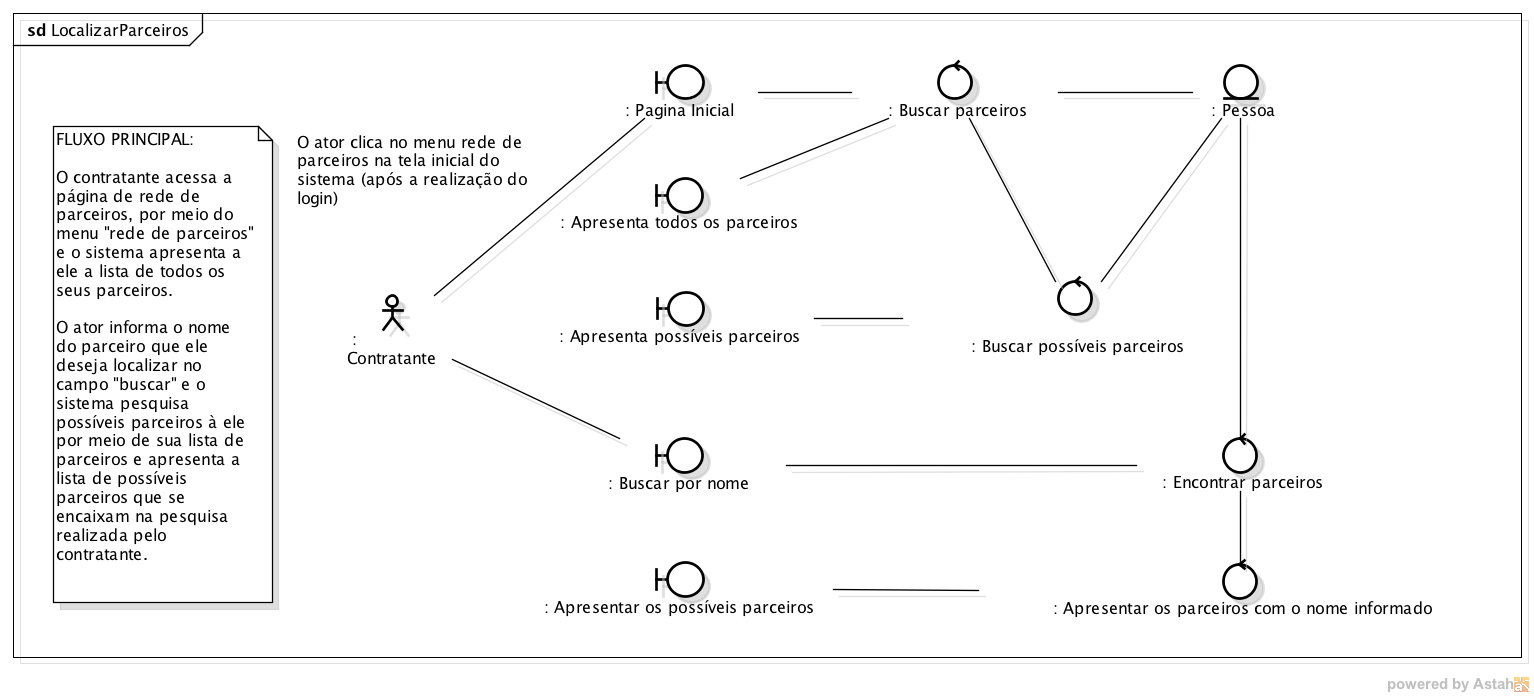
\includegraphics[scale=0.35]{./imagens/apendices/diagrama-robustez-localizar-parceiros.png}}
	\caption[Diagrama de robustez do caso de uso ''Localizar parceiros'']
	{Diagrama de robustez do caso de uso ''Localizar parceiros''. \textbf{Fonte:} Elaborado pelos autores.}
	\label{fig:diagrama_robustez_localizar_mao_de_obra}
\end{figure}

Em paralelo, foi atualizado o modelo de domínio, acrescentando os novos atributos identificados na segunda fase, conforme a Figura~\ref{fig:modelo_dominio_atualizado}.

\newpage
\begin{figure}[h!]
	\centerline{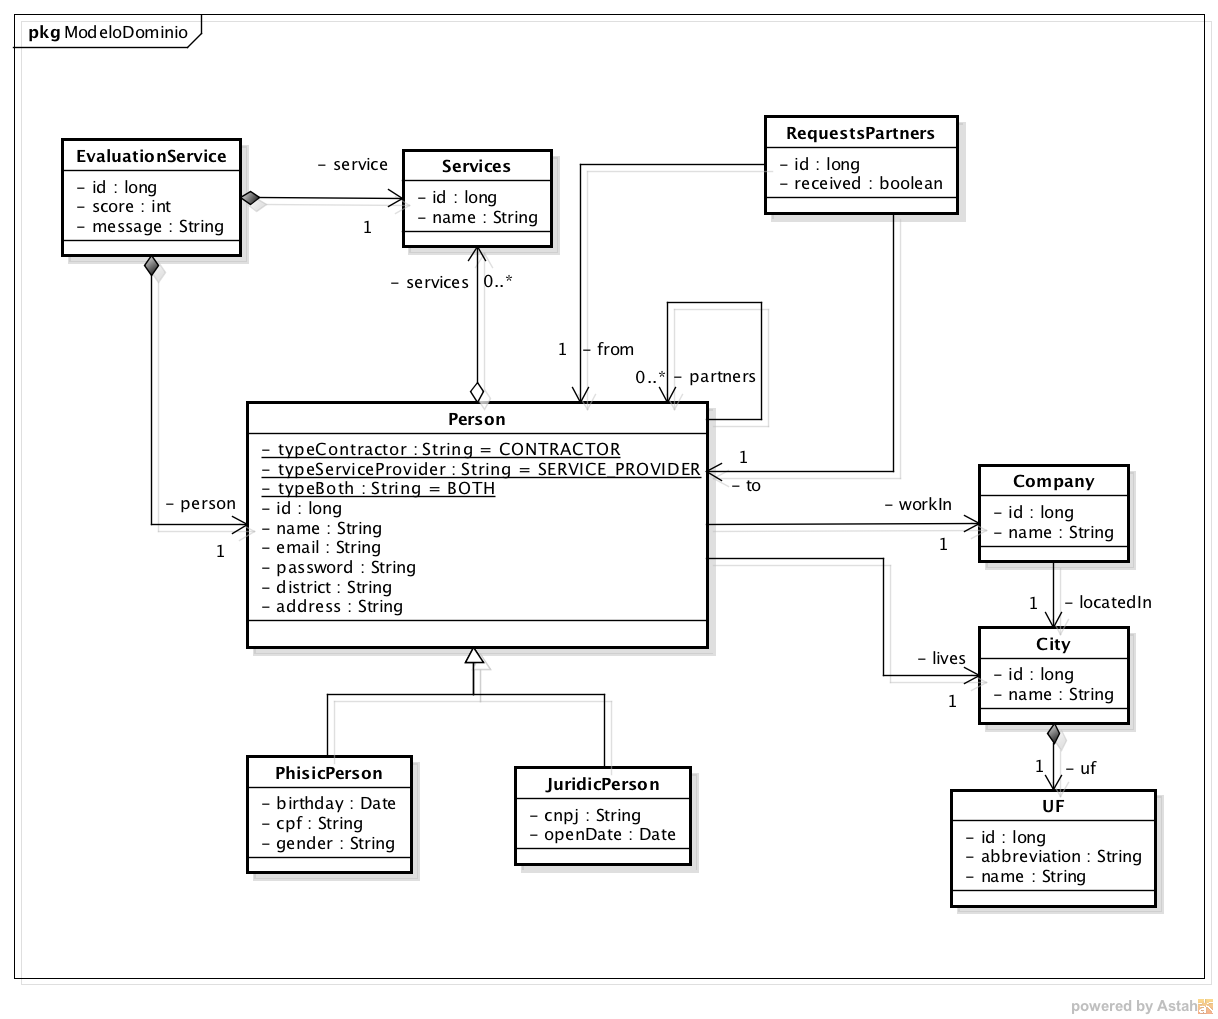
\includegraphics[scale=0.5]{./imagens/modelo-dominio-com-atributos.png}}
	\caption[Modelo de domínio atualizado]
	{Modelo de domínio atualizado. \textbf{Fonte:} Elaborado pelos autores.}
	\label{fig:modelo_dominio_atualizado}
\end{figure}

Com o modelo de domínio atualizado, foi feita a modelagem do banco de dados da aplicação, como apresenta a Figura~\ref{fig:modelo_dados_aplicacao}.

\newpage
\begin{figure}[h!]
	\centerline{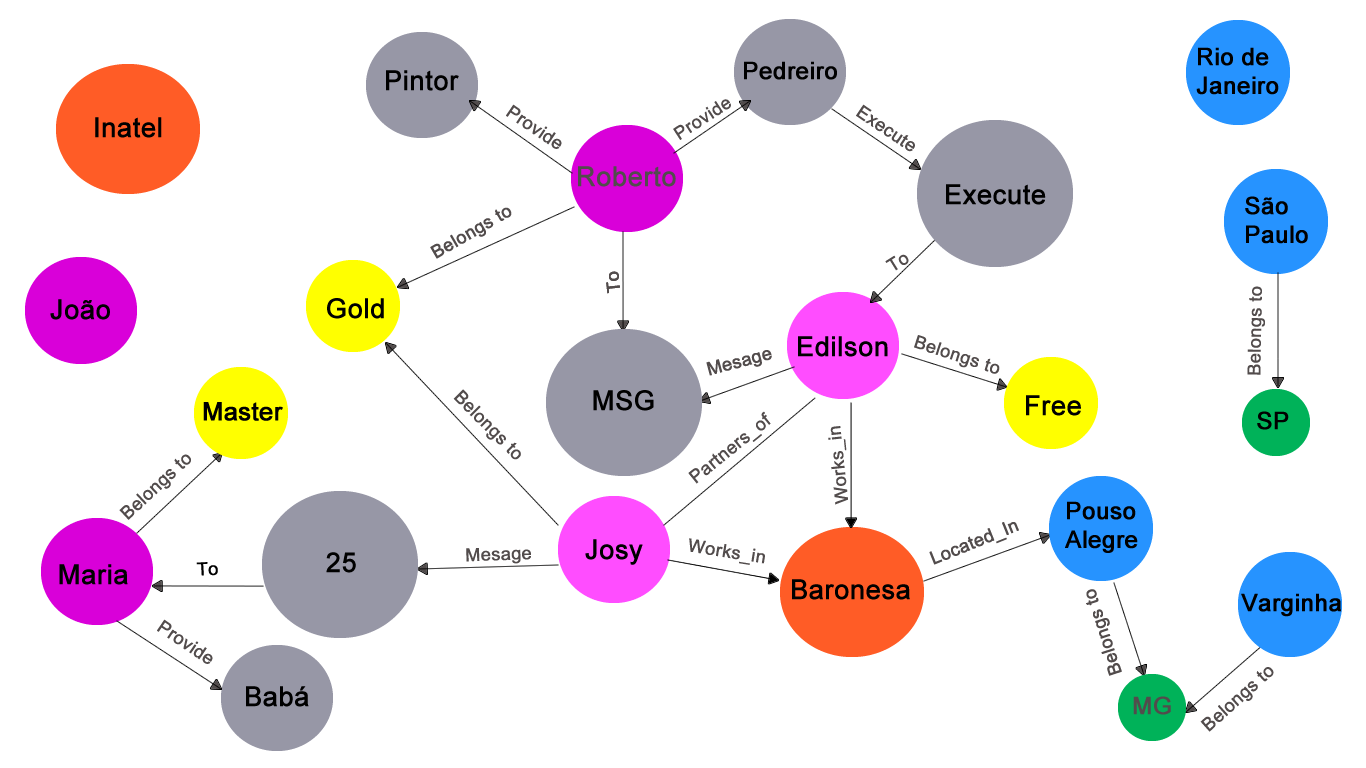
\includegraphics[scale=0.3]{./imagens/structure-all-nodes.png}}
	\caption[Modelo de dados da aplicação]
	{Modelo de dados da aplicação. \textbf{Fonte:} Elaborado pelos autores.}
	\label{fig:modelo_dados_aplicacao}
\end{figure} 

\par Na terceira fase, definida como projeto detalhado, foram criados os diagramas de sequência, tendo como base os casos de uso modelados na fase anterior. Esta fase tem como objetivo detalhar todo o funcionamento do \textit{software}, visando definir a melhor maneira de realizar sua implementação. A Figura~\ref{fig:diagrama_sequencia_localizar_parceiros} apresenta o diagrama de sequência do caso de uso ''Localizar parceiros''.

\newpage
\begin{figure}[h!]
	\centerline{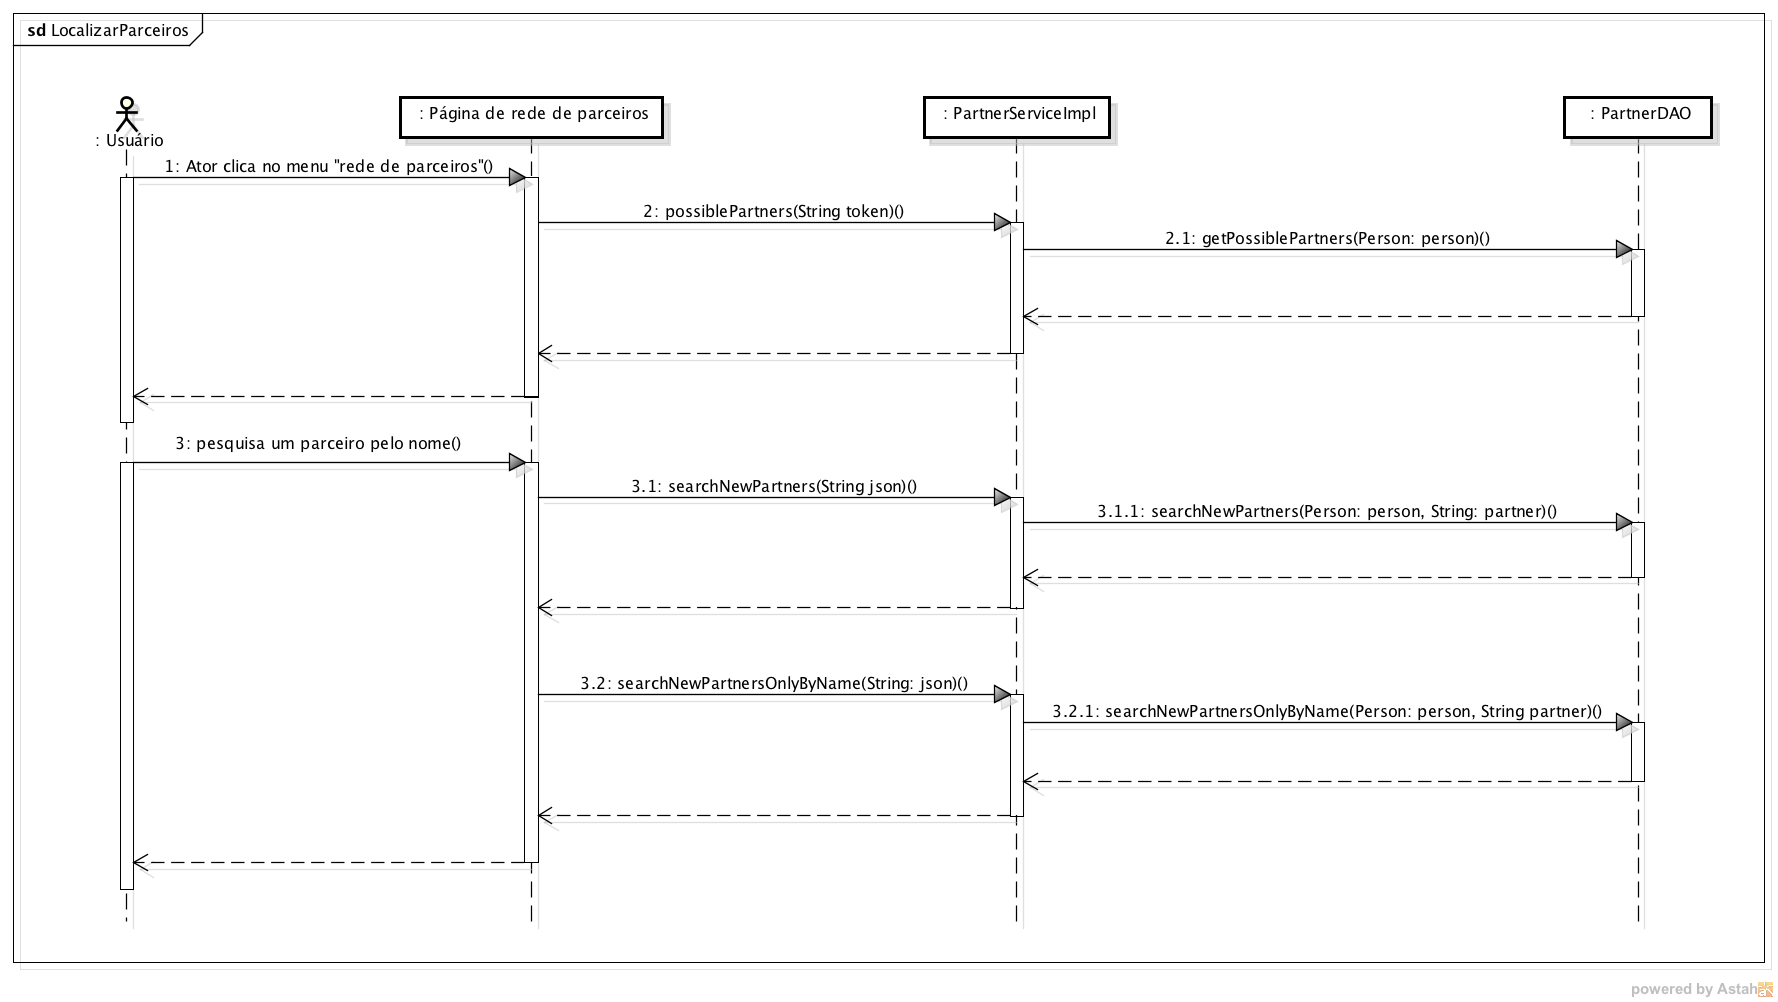
\includegraphics[angle=90,scale=0.4]{./imagens/apendices/diagrama-sequencia-localizar-parceiros.png}}
	\caption[Diagrama de sequência do caso de uso ''Localizar parceiros'']
	{Diagrama de sequência do caso de uso ''Localizar parceiros''. \textbf{Fonte:} Elaborado pelos autores.}
	\label{fig:diagrama_sequencia_localizar_parceiros}
\end{figure}

\par Ainda na fase de projeto detalhado, após a modelagem dos diagramas de sequência, as operações encontradas neles foram adicionadas ao modelo de domínio, em conjunto com as novas classes identificadas, gerando assim, o digrama de classes como mostra a Figura~\ref{fig:diagrama_classe}.

\newpage
\begin{figure}[h!]
	\centerline{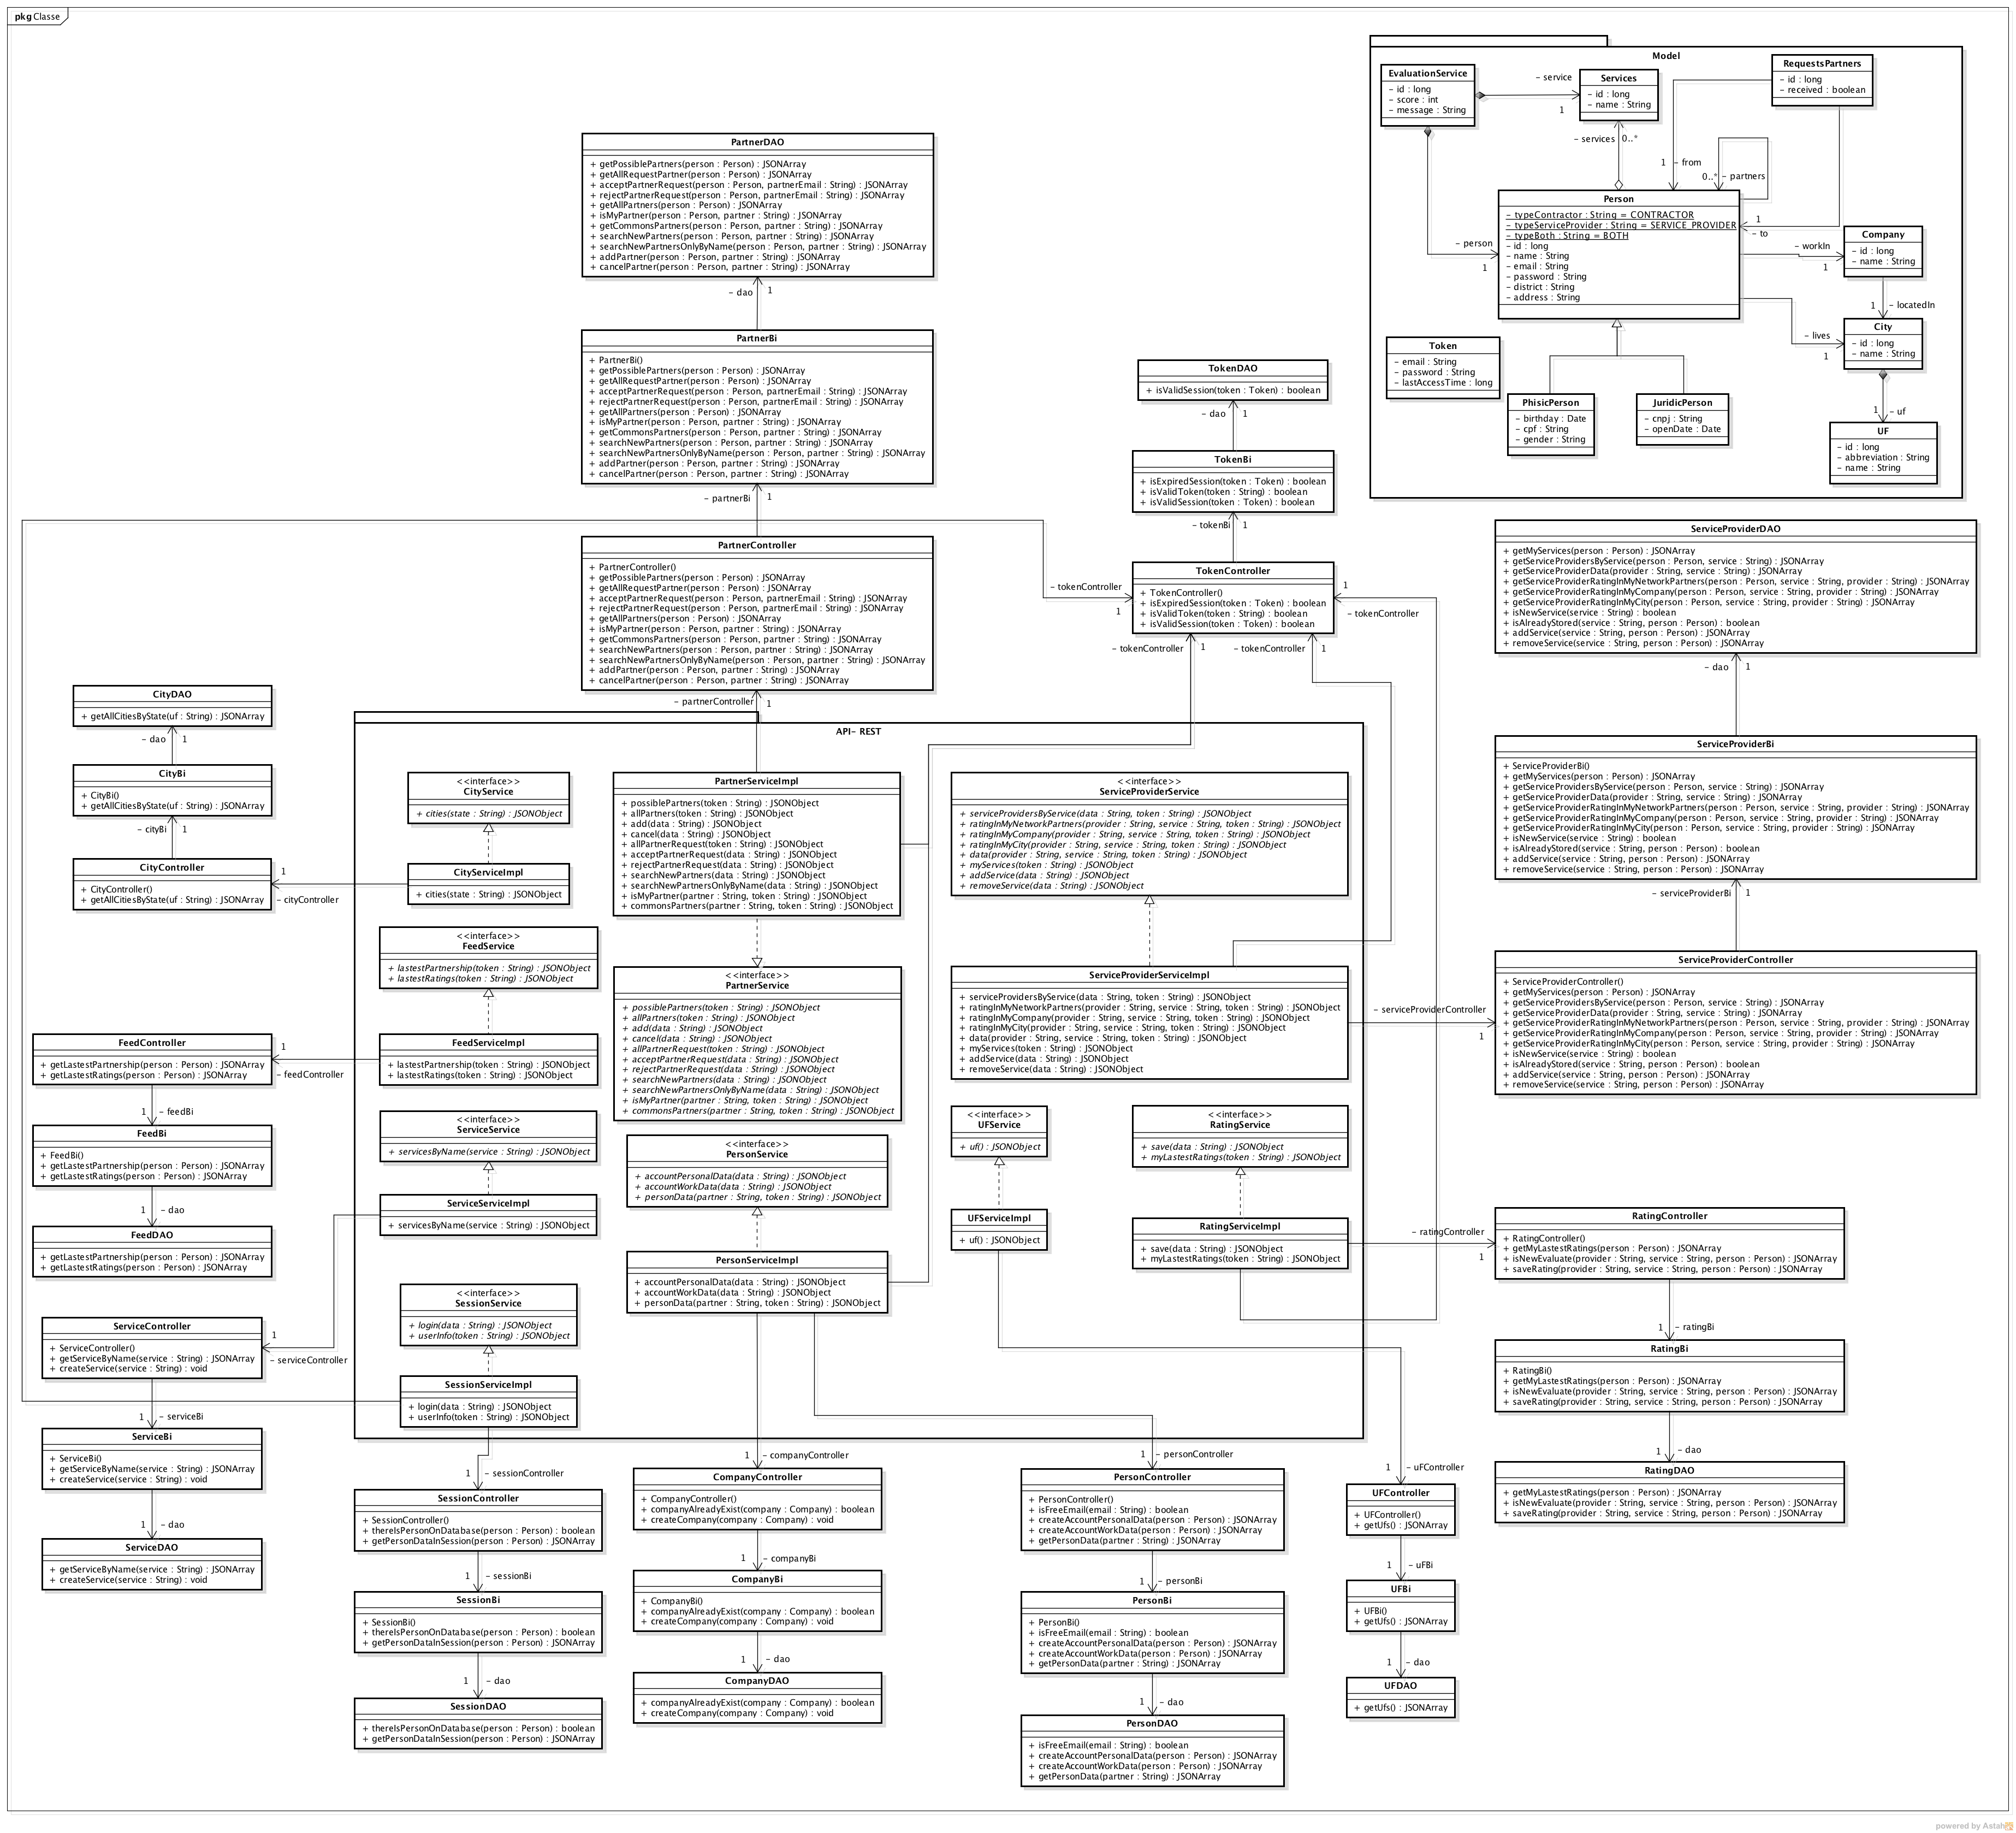
\includegraphics[scale=0.17]{./imagens/classe-full.png}}
	\caption[Diagrama de classes.]
	{Diagrama de classes. \textbf{Fonte:} Elaborado pelos autores.}
	\label{fig:diagrama_classe}
\end{figure}

\newpage
\par Na quarta e última fase do ICONIX, denominada implementação, iniciou-se a preparação do ambiente, incluindo a instalação dos \textit{softwares} necessários para o desenvolvimento prático da aplicação. Essa preparação é abordada a seguir.
